\begin{frame}{Fitting a Line to Data}
    In this section, we will talk about fitting a line to data.
    \begin{itemize}
        \item Linear regression will allow us to look at relationships between two (or more) variables.
        \item This is a bit like ANOVA, but now we will be able to \textit{predict} outcomes.
    \end{itemize}
\end{frame}

\begin{frame}{Fitting a Line to Data}
    \begin{center}
        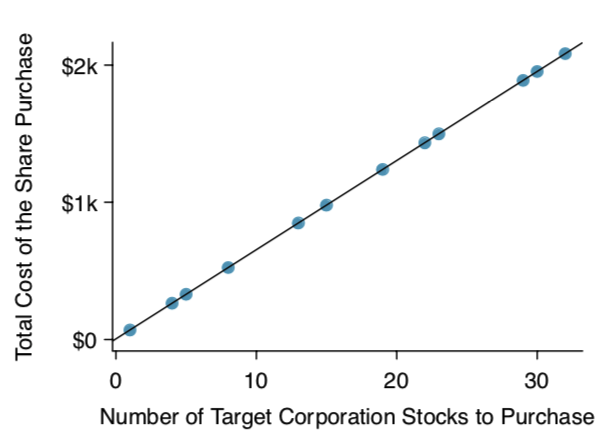
\includegraphics[scale=0.35]{images/perfectcorr.png}
    \end{center}
    This relationship can be modeled perfectly with a straight line:
    \[
        y = 5 + 64.96x
    \]
    I.e., $x$ and $y$ are perfectly correlated.
\end{frame}

\begin{frame}{Fitting a Line to Data}
    When we can model a relationship \textit{perfectly},
    \[
        y = 5 + 64.96x,
    \]
    we know the exact value of $y$ just by knowing the value of $x$.
    
    \vspace{12pt}However, this kind of perfect relationship is pretty unrealistic... it's also pretty uninteresting.
\end{frame}

\begin{frame}{Linear Regression}
    Linear regression takes this idea of fitting a line and allows for some error:
    \[
        y = \beta_0 + \beta_1 x + \epsilon
    \]
    \begin{itemize}
        \item $\beta_0$ and $\beta_1$ are the model's parameters.
        \item The error is represented by $\epsilon$.
    \end{itemize}
\end{frame}

\begin{frame}{Linear Regression}
    \begin{itemize}
        \item The parameters $\beta_0$ and $\beta_1$ are estimated using data.
        \item We denote these point estimates by $b_0$ and $b_1$.
        \begin{itemize}
            \item ...or sometimes $\hat{\beta}_0$ and $\hat{\beta}_1$
        \end{itemize}
    \end{itemize}
\end{frame}

\begin{frame}{Linear Regression}
    For a regression line
    \[
        y = \beta_0 + \beta_1 x + \epsilon
    \]
    we make predictions about $y$ using values of $x$.
    \begin{itemize}
        \item $y$ is called the \textbf{response variable}.
        \item $x$ is called the \textbf{predictor variable}. 
    \end{itemize}
\end{frame}

\begin{frame}{Linear Regression}
    When we find our point estimates $b_0$ and $b_1$, we usually write the line as
    \[
        \hat{y} = b_0 + b_1 x
    \]
    We drop the error term because it is a random, unknown quantity. Instead we focus on $\hat{y}$, the predicted value for $y$. 
\end{frame}

\begin{frame}{Linear Regression}
    As with any line, the intercept and slope are meaningful.
    \begin{itemize}
        \item The slope $\beta_1$ is the change in $y$ for every one-unit change in $x$.
        \item The intercept $\beta_0$ is the predicted value for $y$ when $x=0$.
    \end{itemize}
\end{frame}

\begin{frame}{Clouds of Points}
        \centering
        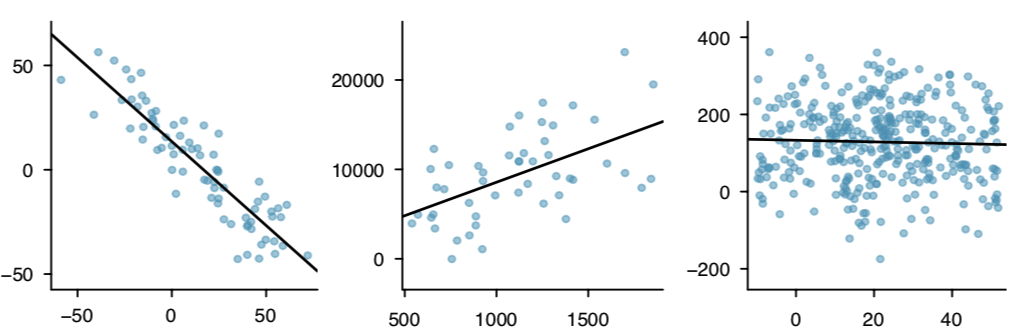
\includegraphics[width=4.5in]{images/ptclouds.png}
\end{frame}

\begin{frame}{Clouds of Points}
    Think of this like the 2-dimensional version of a point estimate.
    \begin{itemize}
        \item The line gives our best estimate of the relationship.
        \item There is some variability in the data that will impact our confidence in our estimates.
        \item The true relationship is unknown.
    \end{itemize}
\end{frame}

\begin{frame}{Linear Trends}
    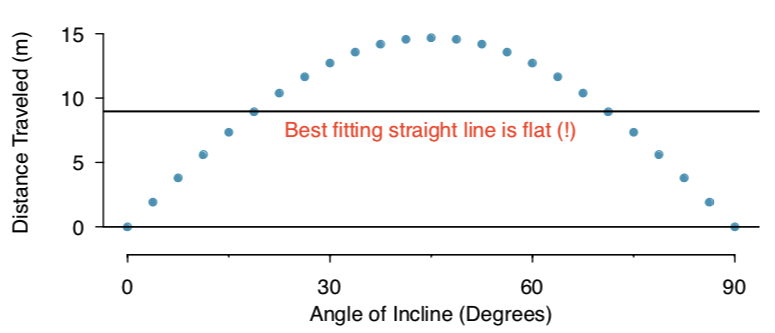
\includegraphics[scale=0.4]{images/curvereg.png}
    \vspace{1cm}
    
    Sometimes, there is a clear relationship but simple linear regression won't work! We will talk about this later in the term.
\end{frame}

\begin{frame}{Prediction}
    Often, when we build a regression model our goal is prediction.
    \begin{itemize}
        \item We want to use information about the predictor variable to make predictions about the response variable.
    \end{itemize}
\end{frame}

\begin{frame}{Example: Possum Head Lengths}
    \begin{center}
        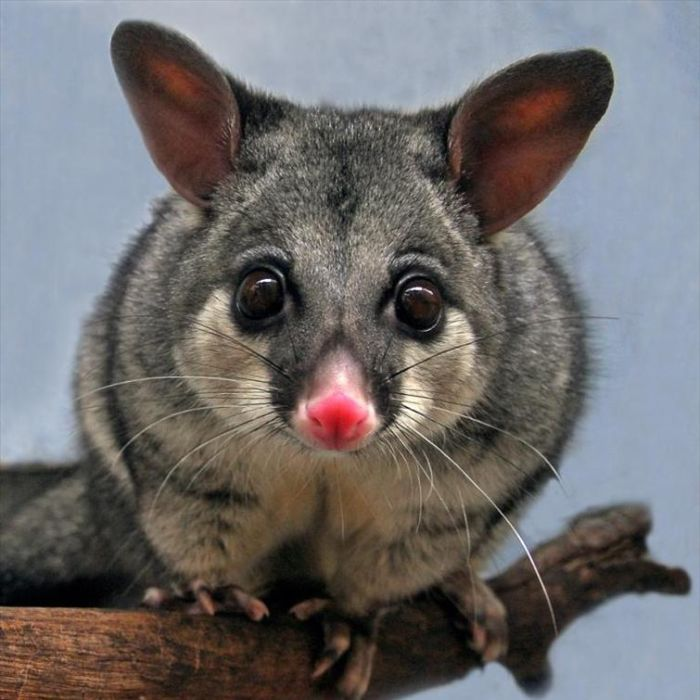
\includegraphics[scale=0.25]{images/possum.jpg}
    \end{center}
    Remember our brushtail possums?
\end{frame}

\begin{frame}{Example: Possum Head Lengths}
    Researchers captured 104 brushtail possums and took a variety of body measurements on each before releasing them back into the wild.
    
    \vspace{12pt}We consider two measurements for each possum:
    \begin{itemize}
        \item total body length.
        \item head length.
    \end{itemize}
\end{frame}

\begin{frame}{Example: Possum Head Lengths}
    \begin{center}
        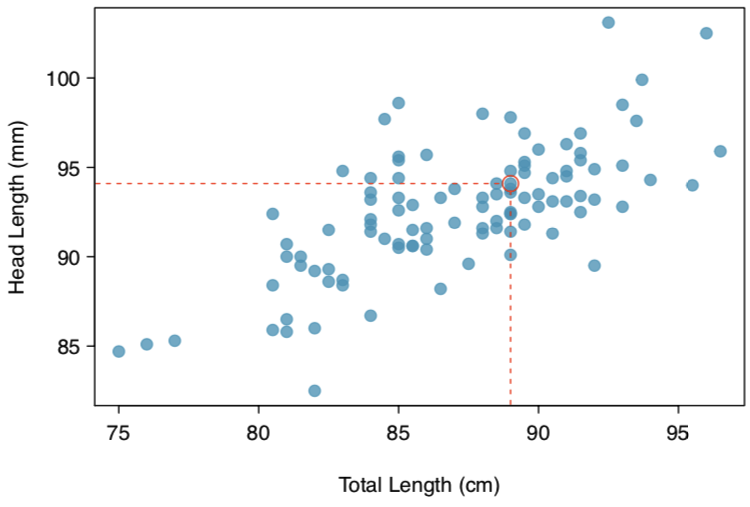
\includegraphics[scale=0.35]{images/possumscatter.png}
    \end{center}
\end{frame}

\begin{frame}{Example: Possum Head Lengths}
    \begin{itemize}
        \item The relationship isn't perfectly linear.
        \item However, there does appear to be a linear relationship.
        \item We want to try to use body length to predict head length.
    \end{itemize}
\end{frame}

\begin{frame}{Example: Possum Head Lengths}
    The textbook gives the following linear relationship:
    \[
        \hat{y} = 41 + 0.59x
    \]
    As always, the hat denotes an estimate of some unknown true value. 
\end{frame}

\begin{frame}{Example: Possum Head Lengths}
    \begin{center}
        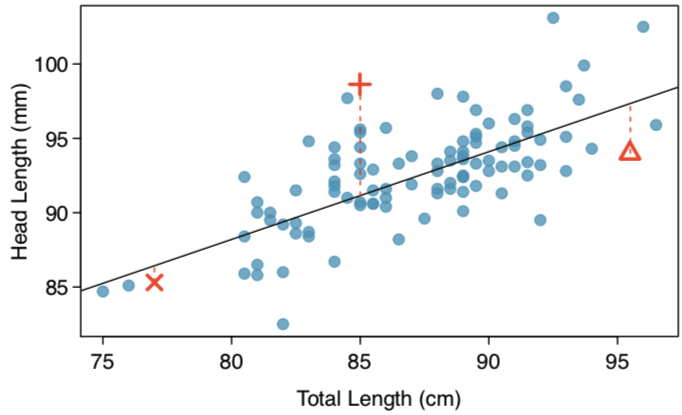
\includegraphics[scale=0.35]{images/possreg.png}
    \end{center}
    Predict the head length for a possum with a body length of 80 cm. 
\end{frame}

\begin{frame}{Example: Possum Head Lengths}
    If we had more information (other variables), we could probably get a better estimate. 
    
    \vspace{12pt}We might be interested in including
    \begin{itemize}
        \item sex
        \item region
        \item diet
    \end{itemize}
    or others.
    
    \vspace{12pt}Absent addition information, our prediction is a reasonable estimate.
\end{frame}

\begin{frame}{Residuals}
    \textbf{Residuals} are the leftover variation in the data after accounting for model fit:
    \[
        \text{data} = \text{prediction} + \text{residual}
    \]
    Each observation will have its own residual.
\end{frame}

\begin{frame}{Residuals}
    Formally, we define the residual of the $i$th observation $(x_i,y_i)$ as the difference between observed ($y_i$) and expected ($\hat{y}_i$):
    \[
        e_i = y_i - \hat{y}_i
    \] 
    We denote the residuals by $e_i$ and find $\hat{y}$ by plugging in $x_i$.
\end{frame}

\begin{frame}{Residuals}
    If an observation lands above the regression line,
    \[
        e_i = y_i - \hat{y}_i > 0.
    \]
    If below,
    \[
        e_i = y_i - \hat{y}_i < 0.
    \]
\end{frame}

\begin{frame}{Residuals}
    When we estimate the parameters for the regression, our goal is to get each residual as close to 0 as possible.
\end{frame}

\begin{frame}{Example: Possum Head Lengths}
    \begin{center}
        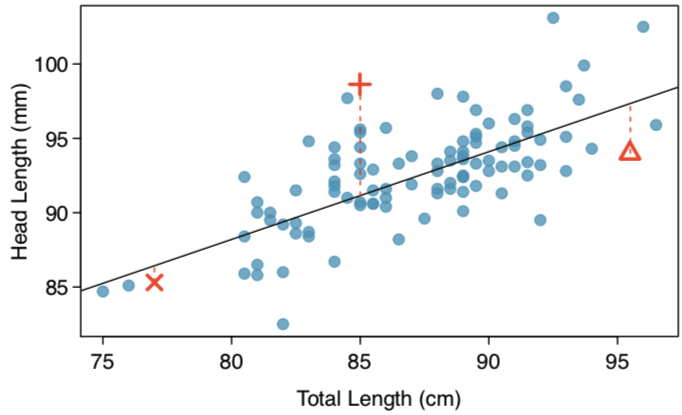
\includegraphics[scale=0.3]{images/possreg.png}
    \end{center}
    The residual for each observation is the vertical distance between the line and the observation. 
\end{frame}

\begin{frame}{Example: Possum Head Lengths}
    The scatterplot is nice, but a calculation is always more precise. Let's find the residual for the observation $(77.0, 85.3)$.
\end{frame}

\begin{frame}{Residual Plots}
    \begin{itemize}
        \item Our goal is to get our residuals as close as possible to 0.
        \item Residuals are a good way to examine how well a linear model fits a data set.
        \item We can examine these quickly using a residual plot.
    \end{itemize}
\end{frame}

\begin{frame}{Residual Plots}
    \begin{center}
        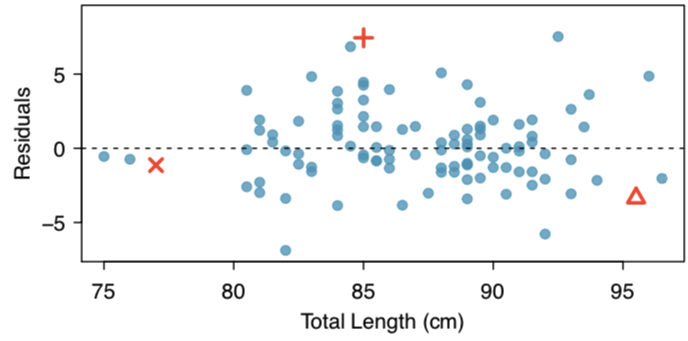
\includegraphics[scale=0.4]{images/resid.png}
    \end{center}
    Residual plots show the $x$-values plotted against their residuals.
\end{frame}

\begin{frame}{Residual Plots}
    \begin{itemize}
        \item We use residual plots to identify characteristics or patterns.
        \item These are things that are still apparent event after fitting the model.
        \item Obvious patterns suggest some problems with our model fit.
    \end{itemize}
\end{frame}

\begin{frame}{Residual Plots}
    \begin{center}
        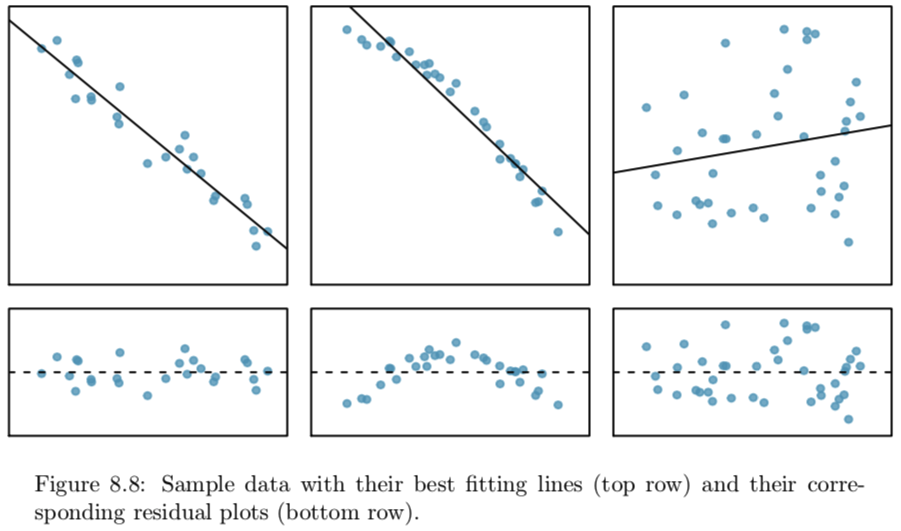
\includegraphics[scale=0.3]{images/residplots.png}
    \end{center}
\end{frame}

\begin{frame}{Correlation}
    We've talked about the strength of linear relationships, but it would be nice to formalize this concept.
    
    \vspace{12pt}The \textbf{correlation} between two variables describes the strength of their linear relationship. It always takes values between -1 and 1. 
\end{frame}

\begin{frame}{Correlation}
    We denote the correlation (or correlation coefficient) by $R$:
    \[
        R = \frac{1}{n-1}\sum_{i=1}^{n}\left(\frac{x_i - \bar{x}}{s_x}\times\frac{y_i - \bar{y}}{s_y}\right)
    \]
    where $s_x$ and $s_y$ are the respective standard deviations for $x$ and $y$.
\end{frame}

\begin{frame}{Correlation}
    Correlations
    \begin{itemize}
        \item Close to -1 suggest strong, negative linear relationships.
        \item Close to +1 suggest strong, positive linear relationships.
        \item Close to 0 have little-to-no linear relationship. 
    \end{itemize}
\end{frame}

\begin{frame}{Correlation}
    Note: the sign of the correlation will match the sign of the slope!
    \begin{itemize}
        \item If $R < 0$, there is a downward trend and $b_1 < 0$.
        \item If $R > 0$, there is an upward trend and $b_1 > 0$.
        \item If $R \approx 0$, there is no relationship and $b_1 \approx 0$.
    \end{itemize}
\end{frame}

\begin{frame}{Correlation}
    \begin{center}
        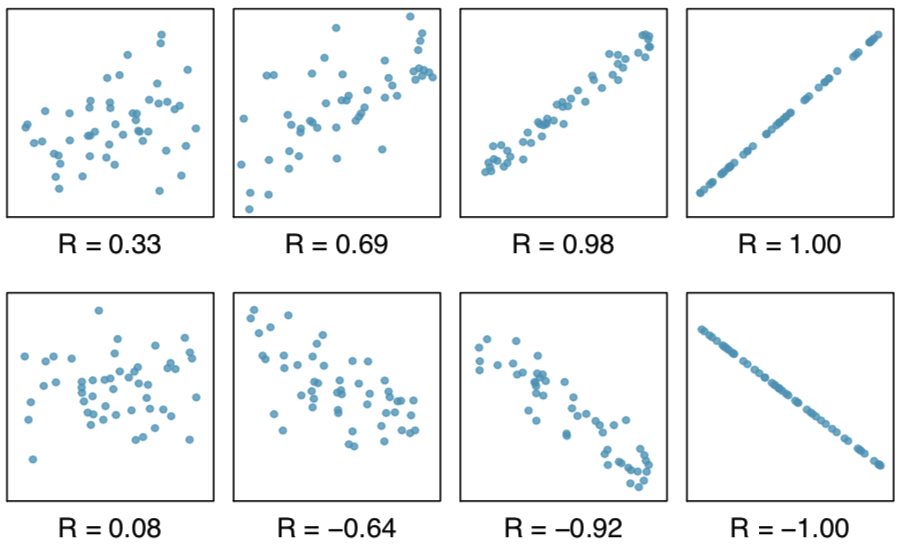
\includegraphics[scale=0.35]{images/correlations.png}
    \end{center}
\end{frame}

\begin{frame}{Correlations}
    Correlations only represent \textit{linear} trends!
    \begin{center}
        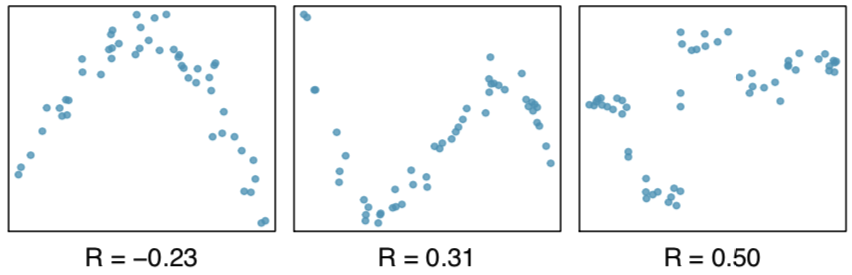
\includegraphics[scale=0.4]{images/nonlincor.png}
    \end{center}
\end{frame}
